\documentclass[12pt]{article}
\usepackage{graphicx}
\usepackage{fancyhdr}
\usepackage{hyperref}
\usepackage{graphicx}
\usepackage{verbatim}
\usepackage{float}
\usepackage{hyperref}
\usepackage{xcolor} 
\usepackage[a4paper, margin=3cm]{geometry}
\pagestyle{fancy}
\fancyhf{} % Efface les en-têtes et pieds de page existants
\fancyhead[L]{\leftmark} % Affiche le titre de la section à gauche de l'en-tête
\fancyhead[C]{} % Centre vide (peut être modifié ou supprimé)
\fancyhead[R]{} % À droite vide (peut être modifié ou supprimé)


\begin{document}

\newcommand{\HRule}{\rule{\linewidth}{0.5mm}}
\newcommand\myfontsize{\fontsize{12.5pt}{1pt}\selectfont}

\begin{titlepage}
    \begin{center}
        Gaea21\\
        Département Observatoire (équipe statistiques)
        \vspace{2.5cm}

        \vspace{0.15cm}
        %\includegraphics[width=5.5cm]{logo_univ_T2.jpg}\\
        \vspace{5cm}
        \HRule
        \vspace{0.5cm}\\
        \textsc{\myfontsize{Rapport de transmission de Basma Ghaffour}}
        \vspace{0.5cm}\\
        \HRule
        \vspace*{0.5cm}


        \begin{minipage}[t]{0.45\textwidth}
            \raggedright 
     
        \end{minipage}
        \hfill % Cette commande ajoute un espace horizontal flexible pour séparer les minipages
        \begin{minipage}[t]{0.45\textwidth}
            \raggedleft
            \large 
            
        \end{minipage}
        \vspace{0.5cm}

        \vfill % Remplit l'espace vertical restant pour pousser la date en bas

        \large{1 juillet 2024 - 27 septembre 2024}
    \end{center}
\end{titlepage}


\newpage


\tableofcontents

\newpage


\section{Introduction}
Dans ce rapport de transmission, je présenterai tout d'abord le projet sur lequel 
j'ai travaillé durant mon stage au sein de Gaea21. J'expliquerai également ce que 
j'ai pu réaliser et ce qui reste à faire pour finaliser le projet qui m'a été attribué. 
Étant donné la complexité des tâches effectuées, j'ai choisi de fournir une explication 
pour chaque tâche dans une sous-section de la section "Explication des projets". À la fin 
de chacune d'elles, j'énoncerai ce qu'il reste à faire afin que les tâches restantes soient
 le plus compréhensibles possible. Dans ce rapport, je suis allé dans les détails techniques 
 afin que le prochain collaborateur puisse reprendre le projet dans les meilleures conditions.



\section{Explication des projets}

J'ai travaillé sur un seul projet durant mon stage,
 ce rapport détaillera ce projet en particulier. \newline

 Afin d'expliquer le projet, les résultats déjà obtenus, 
 ainsi que les tâches que j'ai effectuées, j'ai choisi 
 d'intégrer dans ce rapport de transmission des extraits 
 de mon mémoire de stage et du support de présentation de 
 ma soutenance. J'ai évidemment pris soin de citer les sources 
 lorsque cela était nécessaire et de les ajouter à la bibliographie 
 des documents utilisés pour rédiger ce rapport et pour la 
 réalisation de ce projet en général.\newline

"Lors de la réalisation du stage au sein de Gaea21 le projet 
qui m'a été attribuer est 
intitulé "Trends".
L'objectif de ce projet
est de pouvoir proposer des informations au grand public sur le développement durable. 
Ces informations seront proposées sur le site de Gaea21. Le projet comprend 
trois sections. 
Une section intitulé "Politique" qui a pour but d'informer sur 
les programmes et les politiques qui ont été mis en place pour le
développemment durable. 
Une section  "Actions/Programmes" qui comprend les projets 
que la société civile a déja mis en place. 
Une dernière, nommée "Statistique" qui a pour but de proposer 
des informations chiffrées. 
Cette section comprend
15 thèmes qui sont les suivants : Combustible fossile, 
Energie renouvelable,
Transport, Pêche, Déchets, Eau, Agriculture Durable, Finance Durable, Forêt, 
Consommation Durable, Tourisme, Production Durable, Bâtiments, Communauté Durable, 
Villes Durables. \textbf{Lors de ce stage, j'ai eu pour mission l'étude du thème des énergies renouvelables 
de la section "Statistiques". }"\cite{memoir} \newline

Ainsi, dans les prochaines sous-parties de ce rapport de transmission, 
je vous exposerai chacune des tâches que j'ai réalisées.


\subsection{Documentation sur le sujet}

La première démarche qui a été réaliser lors de ce projet est une recherche 
sur les énergies renouvelables afin de comprendre le sujet. 
Cette étape a permis d'identifier ce qu'étaient les énergies renouvelables 
et comment elles pouvaient être catégorisées. 
\textbf{Cette tâche a été entirement réaliser}, les résultats 
de cette documentation sont les suivant:\newline


"Les énergies renouvelables sont des énergies comme l'électricité ou encore 
la chaleur, par exemple, qui ont été obtenues à partir de technologies utilisant 
des sources d'énergie renouvelable. Les sources d'énergie renouvelable sont, 
selon la définition (donnée dans le document \cite{source_enrg} publié par 
les Nations Unies), des énergies primaires qui se renouvellent à un rythme 
supérieur à celui de leur consommation. Cela comprend la géothermie, le soleil, 
le vent, les cours d'eau, etc. Dans l'article \cite{article_UNEP} publié par les 
Nations Unies, une catégorisation des énergies renouvelables est proposée. 
Elle se segmente de la façon suivante : \newline

\begin{itemize}
    \renewcommand{\labelitemi}{-}
\item Énergie solaire :
L'énergie solaire est obtenue à partir de technologies qui 
utilisent comme source d'énergie le soleil (comme le rayonnement ou encore
la chaleur provenant du soleil). Des technologies comme
les panneaux photovoltaïques ou encore les systèmes solaires 
thermiques, par exemple, 
permettent de produire de la chaleur, 
de l'électricité et d'autres formes d'énergie.
\item Énergie éolienne :
L'énergie éolienne provient de technologies qui exploitent l'énergie 
cinétique du vent, que ce soit sur des zones terrestres ou maritimes, 
pour produire de l'électricité. 
\item Énergie géothermique :
L'énergie géothermique est obtenue par l'exploitation de l'énergie thermique 
provenant de l'intérieur de la Terre. Les technologies utilisant
cette énergie permettent de produire de l'électricité ou de la chaleur.
Comme exemple de technologies, nous pouvons citer les pompes à chaleur géothermique ou encore les 
centrales géothermiques.
\item Énergie hydraulique :
L'énergie hydraulique est obtenue en utilisant des technologies qui exploitent l'énergie 
cinétique de l'eau pour générer de l'électricité, comme les centrales hydroélectriques par exemple.
\item Énergie marine :
L'énergie marine est obtenue par l'exploitation de l'énergie cinétique des vagues
 et des courants marins, ainsi que de l'énergie thermique de l'eau marine. 
 Cela permet de produire de l'électricité ou encore de la chaleur. 
 Nous avons l'exemple des centrales marémotrices.
\item Bioénergie :
La bioénergie est obtenue à partir de la biomasse qui comprend plusieurs types 
de matières organiques comme par exemple le bois, les déchets agricoles, etc. 
Cette biomasse peut être convertie en chaleur, en électricité ou en biocarburants."\cite{memoir}
\end{itemize}

Une des tâches particulièrement demandées est de réaliser un mind map (une carte mentale sur le sujet). 
Ce mind map a été réalisé à partir des résultats de la documentation sur le sujet. En fonction des 
données que vous allez exploiter ou non, vous serez sûrement amené à modifier ce mind map. En revanche, 
ce qui doit absolument être conservé, c'est la catégorisation des énergies renouvelables présentée ci-dessus. \textcolor{red}{\textbf{Vous pouvez accéder à ce mind map à partir de ce \href{https://drive.google.com/file/d/1h-JnPC5I5Rs3szj3WYrmqPE9UIVYSerr/view?usp=drive_link}{lien}}} \newline

Pour les collaborateurs qui reprendront ce projet, je vous invite à vous référer aux 
définitions présentées ci-dessus. Cela vous aidera à bien comprendre le sujet et les 
données sur lesquelles vous serez amenés à travailler. Ces données ont été structurées 
en fonction des différentes catégories d'énergies renouvelables.



\subsection{Identifiacation des sources des données}


Toutes les ressources (dans le sens des organismes qui fournissent des données) 
disponibles sur le thème des énergies renouvelables ont été explorées. 
"Cela a permis d'identifier 
et de répertorier tous les organismes donnant accès à des données sur le sujet. 
Il a ainsi été identifié comme source : \newline

\begin{itemize}
    \renewcommand{\labelitemi}{-}
    \item Our World in data (OWID)
    \item Ember Climate (EC)
    \item Energy Institute (EI)
    \item Organisation for Economic Co-operation and Development (OECD)
    \item International Energy Agency (IEA)
    \item Global Carbon Atlas (GCA)
    \item World Bank Group  (WBG)
    \item International Renewable Energy Agency (IRENA)
    \item UN environment programme (Unep)
    \item The shift data portal (DP)

\end{itemize}

Ces organismes donnent accès à des données mais aussi à des études faites à partir de ces dernières. 
Pour certaines, nous avons également à notre disposition la méthodologie utilisée pour la récolte et 
la construction des bases de données. Les bases de données de tous les organismes ne doivent
pas nécessairement être utilisées. Seules les données à l'échelle mondiale (tous pays confondus), 
régionales (par continent), par unions de pays (comme les pays de l'Union Européenne par exemple), 
par niveau de revenu (par exemple un groupe de pays à haut revenu) et nationales ont été conservées. 
En revanche, les données à l'échelle locale ou infranationale n'ont pas été sélectionnées, 
car elles sont trop précises. Afin de présenter les grandes tendances en matière d'énergies 
renouvelables, il est essentiel de ne pas submerger le lecteur avec trop de détail."\cite{memoir}
\textbf{Cette tâche a été entièrement finie. Si vous en trouvez de nouvelles, vous pourrez les rajouter 
à la liste. J'invite également les futurs collaborateurs à se référer à la liste des sources citées 
afin de poursuivre ce travail.}


\subsection{Collecte des données}

Après avoir identifié des données, il a fallu les collecter. À ce jour, 
je n'ai pas exploité toutes les données de toutes les sources identifiées 
précédemment. J'ai particulièrement exploité les données provenant d'OWID, 
accessibles via leur API\cite{API_OWID}. J'ai également commencé à exploiter une base de 
données fournie par Ember Climate, que vous retrouverez dans le dossier de 
travail. \textbf{Je vous conseil de continuer son exploitation}, car elle est très intéressante. 
En effet, j'ai  exploré des données sur la capacité de 
production d'électricité proposées par IRENA, mais aussi OWID et enfin Ember Climate. 
Ember Climate a effectué de nombreuses recherches supplémentaires. De ce fait, il n'y a 
presque aucune valeur manquante et nous avons donc énormément de données pour divers 
pays et surtout pour divers indicateurs (pas seulement la capacité de production). 


\subsection{Création d'une librairie pour explorer les données}

Pour explorer et préparer les bases de données, 
les fonctions de la librairie `Lib\_OWID` ont été utilisées. 
"La création de cette librairie a permis un gain de temps d'une part, en évitant de refaire les 
mêmes commandes pour l'exploration et la préparation de chacune des bases de données. D'une autre 
part, cela a permis d'alléger considérablement les script de préparation des données et de rendre le 
code beaucoup plus lisible. Cette librairie contient plusieurs fonctionnalités parmi elles :

\begin{itemize}
    \renewcommand{\labelitemi}{-} % Change le style des puces
    \item Une fonction qui permet d'analyser le pourcentage de données manquantes par variable.
    \item Une fonction qui nous permet de vérifier pour chaque pays de la base de données que 
    l'observation d’une année n'est pas présente plusieurs fois.
    \item Une fonction qui nous renvoie des statistiques descriptives de la fréquence 
    d'apparition d'un pays dans la base de données. La fréquence d'apparition qui correspond 
    donc aux nombres d'années pour lesquelles nous avons des observations pour le pays en question. 
    Cela nous est utile pour comprendre les données que l'on manipule et pour supprimer les pays 
    avec trop peu d'observations.
    \item Une fonction qui nous renvoie une liste de tous les pays de la base de données dont 
    la fréquence d'apparition est supérieure à un certain nombre que l'on peut choisir. 
    Cette liste nous a permis de filtrer les pays que l'on souhaite conserver dans notre base de données. 
    Si par exemple un pays a une seule observation, le conserver était inutile compte 
    tenu de l'étude qui a été réalisée."\cite{memoir}
\end{itemize}

Ainsi, lorsque vous travaillerez avec des données (de type pandas.DataFrame qui ont pour index le pays et l'année : (country, year)), 
\textbf{vous aurez la possibilité d'utiliser cette librairie.}

\subsection{Préparation/Nettoyage de base de données }

J'ai actuellement préparé 4 bases de données : sur la capacité de production d'électricité des 
énergies renouvelables (capacity), sur l'investissement dans les énergies renouvelables (investments), 
sur le coût (cost) et sur les brevets (patents). Ainsi, il y a déjà 4 bases de données qui ont été 
préparées et restructurées de façon à être directement utilisables. Dans la prochaine sous-section, 
j'expliquerai plus en détail comment ces données ont été restructurées. Ainsi, en fonction des 
nouvelles données que vous exploiterez, \textbf{vous serez amenés à ajouter de nouvelles données préparées au projet.}

\subsection{Création d'indicateurs}

Concernant la création d'indicateur, a ce jours 5 table d'indicateur ont été 
crée elles ont une structure similaire au table des données préparer.
Cette structuration est présenter dans la prochaine sous section.
Les table d'indicateurs crée sont les suivantes:

\begin{itemize}
    \renewcommand{\labelitemi}{-}
    \item 'capacity\_growth\_all\_renewable\_energy' : Cette table contient le taux de variation de la capacité 
    de production d'électricité à partir d'énergies renouvelables d'une année par rapport à l'année précédente. 
    Elle inclut toutes les catégories d'énergies renouvelables confondues.
    \item 'investments\_percentage\_by\_energy' : Cette table présente, pour chaque année et pour 
chaque pays, la répartition des investissements totaux accordés à tous les types d'énergies renouvelables. 
Pour chaque type d'énergie, elle indique le pourcentage des investissements qui lui a été attribué.
    \item 'investments\_growth\_all\_renewable\_energy' : Cette table présente le taux de variation des 
    investissements dans les énergies renouvelables d'une année par rapport à l'année précédente. 
    (tous les types d'énergies renouvelables confondus)
    \item 'patents\_growth\_all\_renewable\_energy': Cette table présente le taux de variation
du nombre de brevets d'une année par rapport à l'année précédente (brevets sur toutes 
les catégories d'énergie renouvelable confondues).
    \item 'patents\_percentage\_by\_energy': Cette table présente, pour chaque année et pour chaque pays,
la répartition des brevets totaux accordés aux différents types d'énergie renouvelable.

\end{itemize}


\subsection{Rescturation des données}

Afin de bien comprendre les données avec lesquelles nous travaillons, mais aussi pour permettre de 
futures jointures et filtres sur ces dernières, toutes les données brutes préparées ont été 
restructurées de façon similaire.\newline

"Toutes les bases de données ont donc deux index nommé ’country` et `year`. 
Ces index à la fin de la préparation des données ont été transformés en variables afin de faciliter le 
filtrage dans les étapes suivantes de l'étude. Ainsi, les bases de données ont toutes comme colonnes :
\begin{itemize}
    \renewcommand{\labelitemi}{-}
    \item 'country' : indique le nom du pays, du continent, de l'union de pays, etc.
    \item 'year : qui indique l'année de l'observation.
    \item 'id' : qui correspond à la concaténation de la variable 'country' et de la variable 'year'. 
    C’est un identifiant unique pour les observations. Par exemple, une observation en France en 2004 
    aura comme id 'France\_2004'. Cet identifiant sera utile pour la suite de l'étude.
    \item 'zone\_type': Nous indique si l'observation est nationale, continentale, correspond à un 
    ensemble de pays ayant un certain niveau de revenu ou à une union de pays comme l'Union européenne.
    \item 'version\_id' : qui indique le nombre de fois que les données ont été mis à jours.
    \item 'version\_date' qui indique la date exacte à laquelle les données ont été mis à jours."\cite{memoir}
\end{itemize}

\subsection{Création de graphique}

Plusieurs graphiques provisoires ont été créés. Vous pouvez les retrouver dans les notebooks ou
directement au format JPG dans le dossier de travail.

\subsection{Processus d'automatisation de l'étude qui a été proposer}

Une des problématiques de ce projet, en plus de celle énoncée dans la partie explicative, 
consiste à automatiser tout le processus de l'étude. 
Ce processus est valable pour l'instant uniquement sur les 4 bases de données que j'ai exploitées. 
L'exploitation de ces 4 bases de données m'a permis de tester et d'élaborer le processus d'automatisation.
\textbf{\textcolor{red}{Il est évident que ce processus va être modifié et va évoluer, et 
je vous invite à améliorer ce qui doit l'être.}} \newline

\subsubsection{Segementation des différentes étapes de l'étude}

Afin d'expliquer comment j'ai réalisé l'automatisation de l'étude, qui est assez complexe à décrire, 
j'ai choisi d'intégrer les schémas que j'ai créés lors de ma présentation pour la soutenance de stage. 
Ainsi, j'intégrerai dans ce rapport des figures provenant de cette présentation (\cite{beamer}).
\textbf{Évidemment, je ne pourrai pas expliquer tout le processus en détail, seulement les grandes lignes. 
J'ai essayé de documenter et de commenter le code autant que possible afin que vous puissiez 
comprendre ce qui a été fait.} \newline


Pour réaliser le processus d'automatisation, j'ai segmenté l'étude en plusieurs parties.
Ces différentes étapes sont présentées sur la figure \ref{fig:seg} ci-dessous :
\begin{figure}[H]
    \centering
    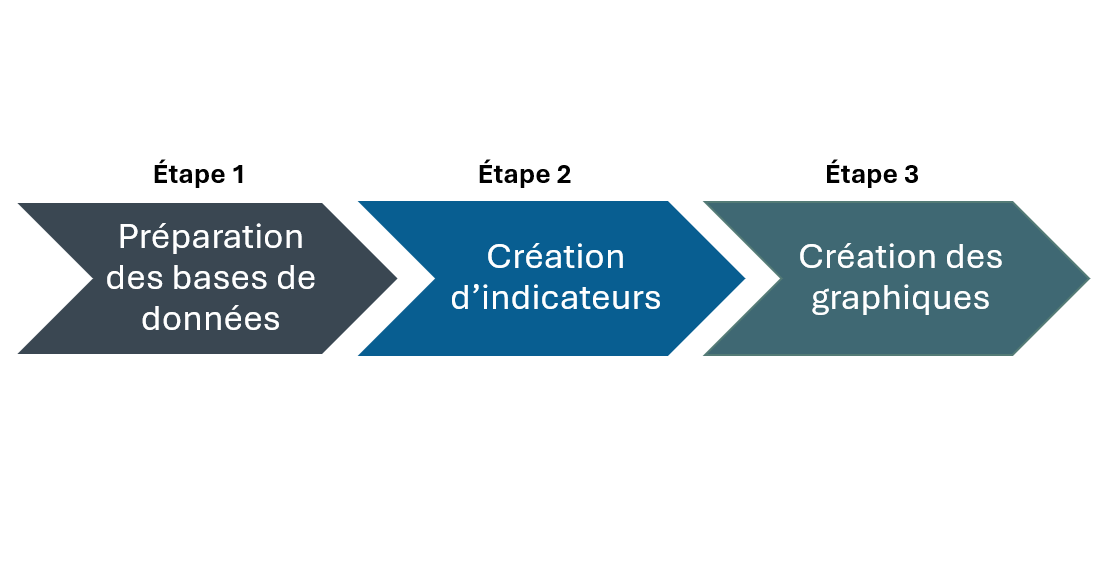
\includegraphics[width=\textwidth]{etape.png}
    \caption{ Différente étapes de l'étude \cite{beamer}}
    \label{fig:seg}
\end{figure}

Afin d'intégrer cette étude dans un processus d'automatisation, j'ai choisi de modulariser les 
scripts Python sur lesquels j'ai travaillé en fonction de ces différentes étapes. 
\textbf{\textcolor{red}{Il est particulièrement important de préciser que l'étape de représentation graphique 
a été réalisée par l'équipe statistique, mais les graphiques sont provisoires et seront 
réalisés par l'équipe IT afin d'être intégrés sur le site.}} Ainsi, les scripts Python du 
processus sont modulés uniquement en fonction des deux premières étapes et des bases de données exploitées.\newline

L'intérêt d'avoir autant modulé les scripts est, d'une part, de rendre le code beaucoup 
plus lisible, mais aussi de faciliter la modification en cas d'erreur. Un travail sur 
la gestion des erreurs a été effectué de manière à ce que, si une erreur se produit, 
elle soit la plus facilement réparable. Cela provient également du fait que les données 
ne sont pas forcément mises à jour au même moment.

\subsubsection{Etape 1}

Tous les scripts Python correspondant à l'étape 1 contiennent le numéro 1 dans leur nom. 
Ces scripts permettent de réaliser différentes actions que vous pouvez visualiser dans 
la figure \ref{fig:etape1} suivante :

\begin{figure}[H]
    \centering
    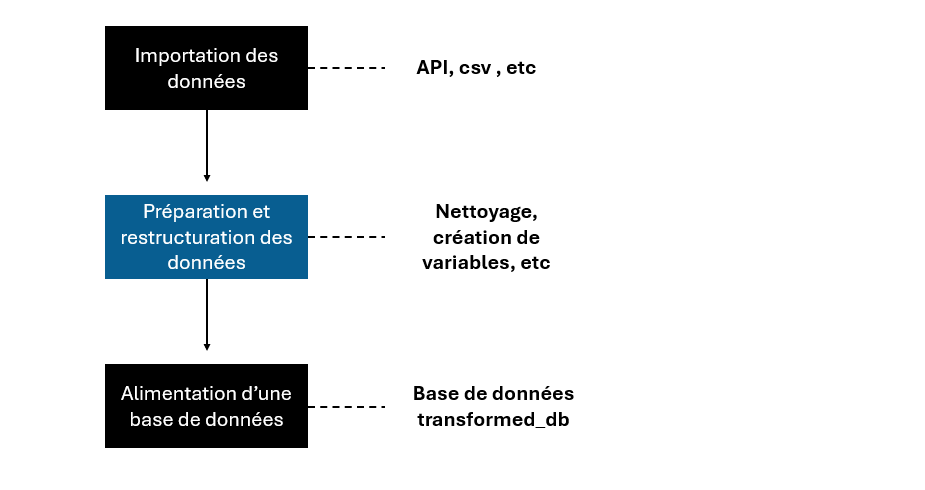
\includegraphics[width=\textwidth]{schema_et1.png}
    \caption{ Etape 1}
    \label{fig:etape1}
\end{figure}


\subsubsection{Etape 2}

Tous les scripts Python correspondant à l'étape 2 contiennent le numéro 2 dans leur nom. 
Ces scripts permettent de réaliser différentes actions que vous pouvez visualiser dans 
la figure \ref{fig:etape2} suivante :



\begin{figure}[H]
    \centering
    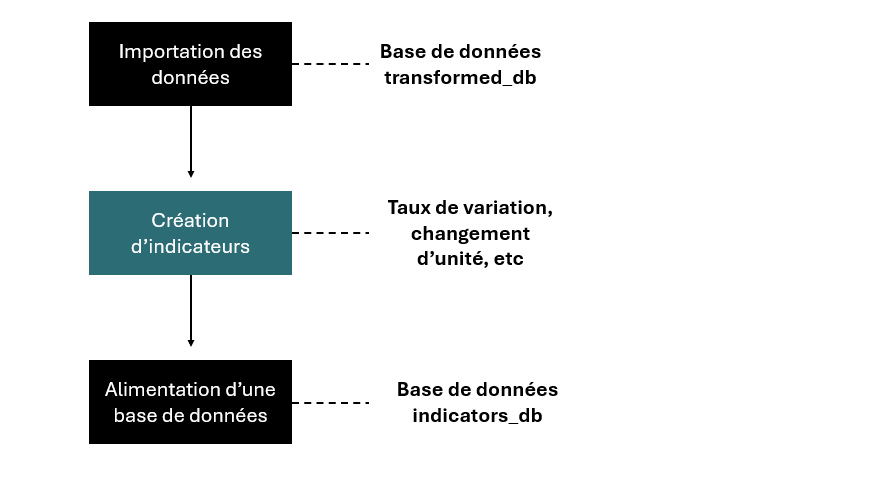
\includegraphics[width=\textwidth]{schema_et2.png}
    \caption{ Etape 2}
    \label{fig:etape2}
\end{figure}


\subsubsection{Flux des données et script du processus d'automatisation}

Comme vous avez pu le constater sur les schémas, on alimente et on importe des 
données provenant de deux bases de données (transformed\_db et indicators\_db). 
Sur la figure \ref{fig:prc} est présenté le processus d'alimentation 
et d'importation des données en fonction des scripts des différentes étapes :

\begin{figure}[H]
    \centering
    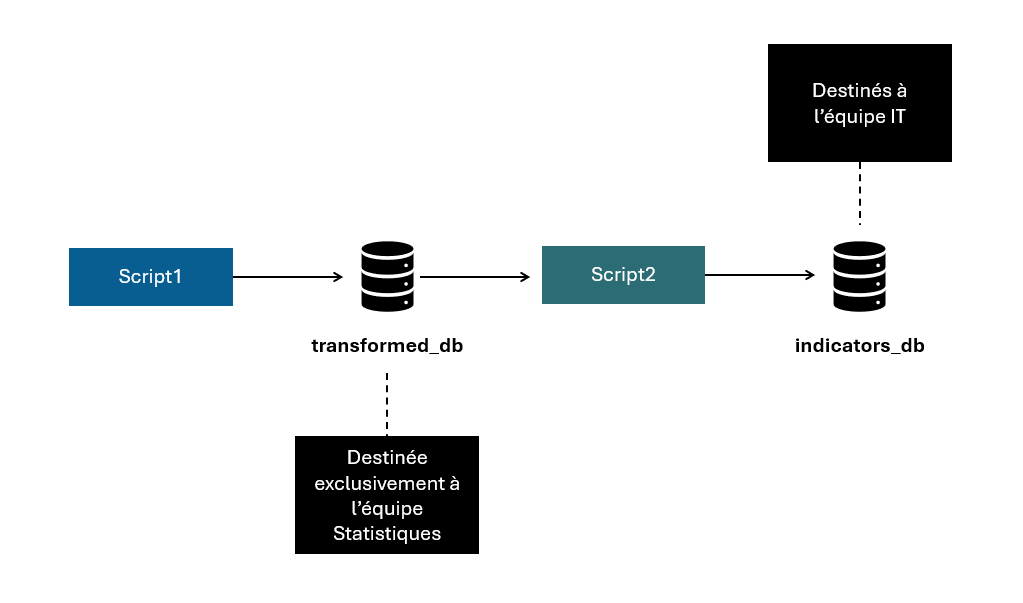
\includegraphics[width=\textwidth]{schema_alim_base.png}
    \caption{ processus d'alimentation et 
    d'importation des données}
    \label{fig:prc}
\end{figure}

On peut facilement constater que les scripts numérotés 1 permettent d'alimenter 
la base de données transformed\_db. Les scripts numérotés 2, quant à eux, importent 
des données de la base de données transformed\_db pour ensuite alimenter la base de données 
indicators\_db.\newline

Le schéma est assez clair, mais il est tout de même important de préciser que 
je n'ai pas vraiment présenté l'idée clairement à l'oral : celle de proposer 
une base de données MySQL destinée exclusivement à l'équipe statistique. 
L'idée initiale, en réalisant ce projet, était de créer une base de données 
MySQL contenant les données brutes qui ont été préparées et structurées de 
manière à être facilement réutilisables par les membres de l'équipe statistique.\newline

En effet, vous serez probablement amenés à réutiliser les données déjà exploitées 
pour créer de nouveaux indicateurs ou pour réaliser des études. Par ailleurs, 
pour que l'équipe IT puisse intégrer les graphiques sur le site, il fallait également 
leur transmettre les données nécessaires à la création de ces graphiques. Ainsi, 
dans ce processus, seules les données indispensables à la réalisation des graphiques 
sont transmises à l'équipe IT.\newline

\underline{Un point important :} \newline
Concernant le schéma de la base de données relationnelle destinée à l'équipe IT, 
des modifications seront nécessaires, notamment pour que la base puisse intégrer 
les données de tous les thèmes. Je ne pourrai pas détailler précisément les 
modifications à apporter, \textbf{\textcolor{red}{textje vous invite donc à vous référer 
à ce \href{https://drive.google.com/file/d/11nOikPpWf0RxfUbokaihUFs0ikDgmV8A/view?usp=sharing}{document} 
et a reprendre la discution avec l'équipe IT.}}


\subsubsection{Détail supplémentaire sur le fonctionement du processus d'automatisation}

Lorsque des données brutes sont mises à jour, ce que l'on souhaite, 
c'est que nos propres données se mettent à jour automatiquement. 
Actuellement, pour les données que j'ai exploitées, je ne sais pas 
quand elles sont mises à jour, et surtout, en raison de la particularité 
de l'API que j'ai utilisée (voir la documentation dans la bibliographie 
concernant l'utilisation du catalogue OWID \cite{API_OWID}), il faudrait manuellement 
explorer à nouveau le catalogue. Si des données plus récentes sont disponibles, 
il faudrait les sélectionner et réexécuter les scripts numérotés 1.\newline

\textbf{Cependant, si l'on importe des données de manière classique ou si l'API évolue, 
il est nécessaire de trouver une méthode pour être alerté de ces mises à jour 
et relancer automatiquement tous les scripts numérotés 1. Il est évident qu'il 
existe une solution simple pour relancer un ensemble de scripts contenant un certain 
terme.} De plus, la relance des scripts numérotés 1 déclenchera automatiquement 
l'exécution des scripts numérotés 2, qui dépendent directement de ces données.\newline

Pour cela, l'utilisation de la librairie subprocess a permis d'automatiser ce processus.  \cite{subprocess}.\newline

\underline{Un point important :}\newline
Ce qu'il reste à faire c'est de trouver des solutions pour alerter lorsqu'il y a 
des modifications et pour relancer un ensemble de scripts. 
\textbf{L'idée de la numérotation et d'une certaine modularité des scripts 
fonctionne bien dans ce que j'ai fait car j'ai créé des indicateurs uniquement 
à partir d'une source de données brutes, mais dans le cas où l'on voudrait créer 
des indicateurs en fonction de plusieurs sources de données brutes, il est possible que 
cette idée ne soit plus d'actualité.}

\subsection{Création d'une librairie pour alimenter une base de données mySQL}

Afin d'alimenter une base de données MySQL, j'ai utilisé les librairies mysql-connector, 
SQLAlchemy et notamment SQLAlchemy.orm. Pour alimenter des tables d'une base de données MySQL, 
une librairie a été créée : alimentation\_table\_mysql. \textbf{Cette librairie est à votre disposition,
elle a été très bien documentée.}\newline

\underline{Un point important :}\newline
La librairie qui permet l'alimentation des tables de données fonctionne très bien, 
a été typée avec mypy, documentée et reformattée avec black. Cependant, je 
n'ai pas eu le temps d'y intégrer les tests avec pytest. Je les ai effectués 
partiellement sur un notebook afin d'intégrer progressivement une gestion des erreurs. 
Ainsi, si vous êtes familier avec pytest (ou d'autres outils), ce qui reste à faire, 
c'est de réaliser les tests.\newline

Dans les prochaines parties de la section sur la création de cette librairie, 
je préciserai quelques outils que j'ai utilisés pour la réaliser.
\subsubsection{Intégration de session pour apporter des modifications}

Afin d'alimenter les tables, j'ai utilisé des sessions dans la librairie. 
Il peut être intéressant pour vous d'utiliser des sessions si vous souhaitez 
réutiliser des tables et apporter des modifications sans que celles-ci soient 
définitives. Pour cela, vous pouvez consulter la documentation suivante : \cite{session}.



\subsubsection{Utilisation de modèle pour sécurisr l'alimentation des données}

Afin d'apporter plus de sécurité au processus d'alimentation des bases de données, 
j'ai utilisé SQLAlchemy.orm pour définir un modèle pour la base de données 
et les tables que j'alimente. Pour mieux comprendre en quoi consiste l'intégration de modèles, 
je vous invite à consulter cette documentation \cite{mapp}. Je vous conseille également, 
si vous n'êtes pas familier avec cette utilisation, de regarder cette
\href{https://www.youtube.com/watch?v=g0-7TrVCNtg}{vidéo} qui explique assez 
bien l'utilisation des modèles et leur intérêt.\newline

Les modèles des deux bases de données MySQL utilisées sont présents dans 
les scripts model\_indicators\_base et model\_transformed\_base. \textbf{Donc, lorsque 
vous voudrez ajouter des tables à l'une ou l'autre des bases de données, 
vous devrez également rajouter le modèle de table en question.}


\subsubsection{Connexion aux bases de données}

Lors de ce projet, j'ai travaillé en local. Donc, lorsque vous récupérerez le projet, 
il faudra créer les deux bases de données avec le même nom (ou alors vous pouvez l’adapter, 
mais pensez à modifier le lien de connexion). Ensuite, tant que les scripts numérotés 
1 n'auront pas été exécutés, vous ne pourrez pas accéder aux tables.\newline

Pour me connecter aux tables, j'ai utilisé MySQL Connector et pour interagir avec les 
tables SQLAlchemy. Pour éviter d'écrire à chaque fois l'URL avec toutes mes informations 
de connexion, j'ai utilisé des variables environnementales qui ont été créées à l'aide de 
la librairie dotenv \cite{dotenve}. \textbf{Vous devrez donc adapter ces variables, qui sont incluses 
dans le fichier .env.}



\subsection{Création d'un environement de travail}

Concernant l'environnement de travail, j'ai utilisé Poetry ainsi qu'un environnement 
virtuel. Ainsi, vous avez seulement à l'activer lorsque vous travaillez sur le projet.
 Cela vous évitera de devoir refaire toutes les configurations.

\section{Conclusion et avis sur le stage}

En conclusion, dans ce rapport de transmission, j'ai présenté brièvement toutes les 
tâches qui ont été effectuées, ainsi que ce qui reste à faire. Le dossier de travail du 
projet doit également être consulté afin de pouvoir comprendre au mieux ce qui a été fait.
\textbf{Je tiens notamment à spécifier une chose : ce projet n'étant pas fini, les éléments 
que j'ai présentés, en fonction de vos avancées, ne seront plus forcément optimaux. Je vous 
invite donc à modifier ce dossier de travail si cela est nécessaire. Cette ébauche du projet 
contient, je pense, l'essentiel de ce qui doit être mis en place et a vocation à être évolutive 
et réutilisable par les futurs collaborateurs. Il est également important de souligner que 
les méthodes utilisées sont des méthodes parmi tant d'autres possibilités, et que 
certaines modifications seront nécessaires à mesure que le projet évoluera. 
La nécessité de prendre en compte cet aspect dès le début a orienté toutes 
les étapes de ce travail.} (\cite{memoir})\newline


"S'agissant de ma première expérience professionnelle dans le domaine et au sein d'une 
association, cette expérience fut très enrichissante. Elle m'a permis d'acquérir de 
nouvelles compétences. Mes études m'ont fourni une base solide pour répondre aux objectifs 
du stage. J'ai pu mobiliser beaucoup des connaissances acquises durant mes études et 
m'adapter aux exigences en approfondissant certains éléments. Notamment grâce à l'utilisation 
de la documentation technique à ma disposition. Cela m'a aidé à trouver des solutions à des 
problèmes auxquels je n'avais pas encore été confronté et a grandement amélioré ma 
capacité à apprendre de manière autonome. J'ai également développé la compréhension 
du processus de création et de réalisation d'un projet, ce qui a été très formateur. 
Cette expérience m'a aussi fait prendre conscience de l'étendue des possibilités 
pour répondre à une exigence, ainsi que des outils et des moyens nécessaires pour y parvenir." 
\cite{memoir} \newline


Je tien à remercier l'association Gaea21 de m'avoir 
accepté en stage. Merci à toute l'équipe de Gaea21, 
du département des ressources humaines, à mes collègues de l'équipe statistique 
et au président de l'association Monsieur Yvan Claude, pour leur accueil. 
Je suis particulièrement reconnaissante envers mon coordinateur, 
Monsieur Jonathan Mauro, pour sa disponibilité, 
pour les réponses qu'il a apportées à mes interrogations,
et pour m'avoir guidé tout au long de ce stage.
Je le remercie également d'avoir pris en compte toutes mes 
suggestions et pour tous les échanges constructifs qu'il m'a permis d'avoir
durant ce stage.


\newpage

\section{bibliographie}
\nocite{*}
\bibliographystyle{plain}
\bibliography{biblio}


\end{document}